\chapter{FITTING THE TENSOR VALUES}
    
    In the previous section, we proposed a way for compressing the indices of a sparsified tensor as those are yielded by the underlying sparsification method.
    However, we never mentioned anything about reducing the size of the tensor values.
    In this section, we will turn our focus on compressing the values of the gradient components instead.
    
    As we already mentioned before, one of the reasons we choose to sparsify the gradient tensors on the first place, is because some of the information they carry is redundant for the training process.
    It has been observed, for example, that many of the values inside those tensors are either zero or extremely close to zero.
    Exchanging all these components between workers would be a significant waste of network resources. 

    \begin{figure}[h]
    \centering
    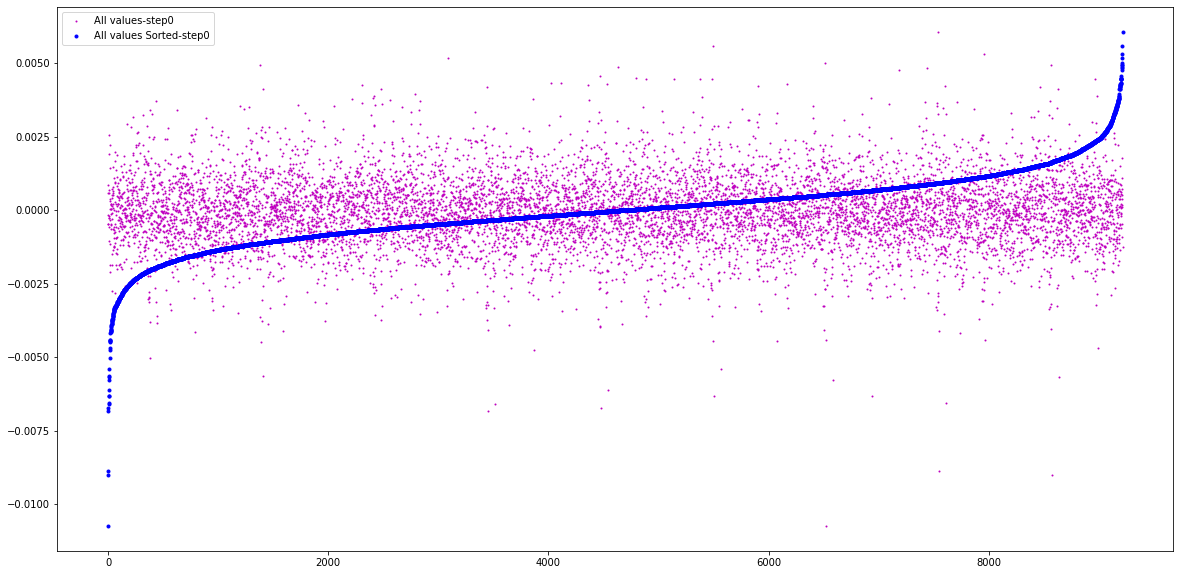
\includegraphics[width=1\textwidth]{thesis/figures/gradient29-step0.png}
    \caption{Resnet20, a gradient of size 9216 at the first step of training}
    \label{gradient29-step0}
    \end{figure}
    
    \begin{figure}[h]
    \centering
    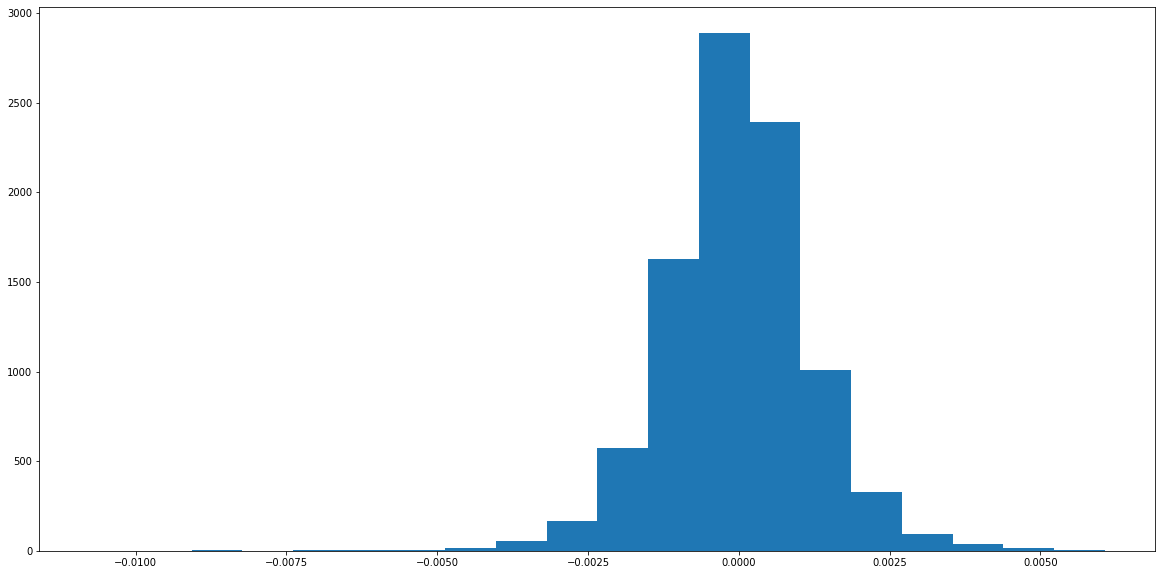
\includegraphics[width=1\textwidth]{thesis/figures/histogram.png}
    \caption{Histogram for the values of the gradient in figure \ref{gradient29-step0}}
    \label{histogram}
    \end{figure}
    
    Another observation is that while the gradient values are densely distributed near zero, they are more and more sparse as we move further away from it.
    This is nicely depicted in figures \ref{gradient29-step0} and \ref{histogram}.
    In figure \ref{gradient29-step0} we have plotted the 9216 values of a gradient as it was generated during the first step of training of resnet20 on the cifar10 dataset.
    Figure \ref{histogram} also shows the histogram of this gradient. 
    It is readily seen, that by sorting those gradient values, we get the blue curve in figure \ref{gradient29-step0} which resembles a function commonly known as "logit" (inverse of sigmoid).
    
    Our goal was to leverage these observations and devise a new method for compressing the gradient values. 
    The idea we propose involves the "curve fitting" process that was described in a previous section.
    
    \section{Encoding/Decoding}

    Let $g\in\R^d$ be the stochastic gradient we want to compress
    and let $g_s\in\R^d$ be the tensor we get after sorting the components of $g$ in an increasing or decreasing order.
    We, then, construct a curve that is an exact fit of the data points $(i, g_s[i]), i=1,2,\cdots,d$.
    That is, we adopt a functional parametric form for this curve and we try to find the optimal, unknown coefficients for which the curve will match this series of points as well as possible. Now, let $m\in\R^d$ be a tensor that keeps information about the mapping of the positions of the initial unsorted gradient components to their new positions in $g_s$.
    For example, the mapping $[1,0,3,2]$ informs us that the value of $g$ in the position $0$ was now placed in the position $1$ inside the sorted tensor $g_s$, the value of $g$ in position $1$ was placed to the position $0$ e.t.c.
    
    Both the coefficients and the mapping must be included in the message that will be communicated to the workers. This way they will be able to reconstruct the curve that approximates the tensor $g_s$ and re-order the estimated values so that they place them in their correct positions. Note that, the parametric form of the function is known both during the compression and the decompression phase.
    Let $f_w$ be this function, where $w$ denotes the coefficients retrieved from the message. 
    Then, every tuple $(m[i], f_w(i)), i=1,2,\cdots,d$ would denote a reconstructed gradient value as well as its position inside the gradient.
    
    It is fair to say, that this whole scheme does not actually decrease the size of the message. On the contrary, if we would just send the gradient components of $g$ without applying any compression, there would be no need to send the mapping, so the message should probably be smaller.
    However, this scheme is only a generalized version of how this compression method is meant to be applied.
    The idea is to use the "values approximation" approach on top of another sparsification method and more specifically, the Top-r method.
    Then, instead of the $r$ values and the $r$ indices needed for the decompression of the sparsified gradient, we would communicate the indices and the coefficients that define the curve, which in practice, will be significantly less than the actual values.
    
    The reason we first establish this more general scheme is to help us investigate how tolerant training is to this compression method and if convergence can be achieved even under the presence of the expected approximation errors.
    
    We will now proceed by describing some of the different approaches we followed for implementing the above encoding/decoding method.


    \section{Linear Regression}
    In linear regression, we assume that the relationship between the dependent output $y$ and the independent inputs  $x_1, x_2, \cdots, x_k$ can be expressed via the following prediction model:
    \begin{flushleft}
    \centering
    \setlength{\parindent}{40ex} 
    $\hat{y} = \hat{w_0} + \hat{w_1}x_1 +  \hat{w_2}x_2 + \cdots + \hat{w_k}x_k := \hat{w}^T x$
    \end{flushleft}
    
    We call this type of regression "linear" because it is indeed linear in the coefficients.
    However, linear regression is not limited to expressing only linear relationships between the output and the input parameters. 
    Indeed, if we raise an independent input variable by any exponent then we can capture non-linear relationships, as well.
    This more generalized prediction model is now written  as follows:
    \begin{flushleft}
    \centering
    \setlength{\parindent}{40ex} 
    $\hat{y} = \hat{w_0} + \hat{w_1}\Phi_1(x_1) +  \hat{w_2}\Phi_2(x_2) + \cdots + \hat{w_k}\Phi_k(x_k)$
    \end{flushleft}
    
    where the $\Phi_j(x)$ are known as basis functions.
    The above can be re-written as:
    \begin{flushleft}
    \centering
    \setlength{\parindent}{40ex} 
    $Y = \sum_{i=0}^k \hat{w_i}\Phi_i(x_i)$
    \end{flushleft}

    assuming that $\Phi_0(x)=1$ so that $w_0$ acts as a bias.
    
    Now, by minimizing the least-squares loss function:
    \begin{flushleft}
    \centering
    \setlength{\parindent}{40ex} 
    $\mathcal{L}_w = \sum_{n=1}^N (y_n-w^T x_n)^2$
    \end{flushleft}
    we obtain the LS estimates for the parameter vector $w$:
    \begin{flushleft}
    \centering
    \setlength{\parindent}{40ex} 
    $\hat{w} = (X^T X)^{-1} X^T y$
    \end{flushleft}
    
    A great advantage of using the LS loss function is that we are able to obtain an analytical solution for computing the coefficients provided that the matrix $X^TX$ is invertible.
    This is a key point for our implementation considering our setting.
    Remember that, we need to solve a regression problem every time we need to compress a gradient and communicate it to the other workers.
    If we had employed more complex models that required iterative mechanisms (e.g. gradient descent) for obtaining the optimal coefficients then the computational overhead of this method would definitely make it unsuitable.
    
    In figure \ref{Regressor}, we see the graph that represents the compressor's computations. 
    The box "LS Regression" abstracts away all the transpose, inverse and matrix multiplication operations that need to take place for computing the coefficients.
    
    \begin{figure}[h]
    \centering
    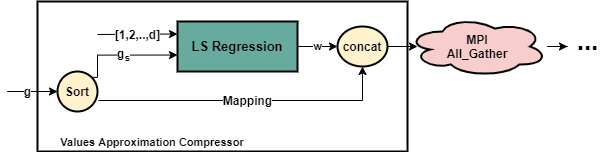
\includegraphics[width=0.9\textwidth]{thesis/figures/regression.png}
    \caption{Values Approximation Compressor}
    \label{Regressor}
    \end{figure}

    \newpage
    Now, by using the LS  model and alternating between different sets of basis functions
    we can create a variety of implementations for the "values approximation" compressor.
    
    As a metric for evaluating the performance of the model we use the Root Mean Squared Error
    which is defined as:
    \begin{flushleft}
    \centering
    \setlength{\parindent}{40ex} 
    $RMSE = \sqrt{\sum_{n=1}^N{\frac{(y_n-w^T x_n)^2}{N}}} $
    \end{flushleft}
    
    \subsection{Logit Functions}

    One of our first attempts was to directly fit the gradient values after those have been sorted in an increasing order.
    The curves shall look like the one in figure \ref{logit}, which, in this case, was computed using linear regression and the simple method of least squares.
    
    As basis functions we used some inverse "sigmoid" functions. \\
    The inverse of a sigmoid is called "logit" and has the following functional form:
    \begin{flushleft}
    \centering
    \setlength{\parindent}{40ex} 
    $\Phi{(x)} = \log{\dfrac{x}{1-x}} $
    \end{flushleft}
    

    \begin{figure}[h]
    \centering
    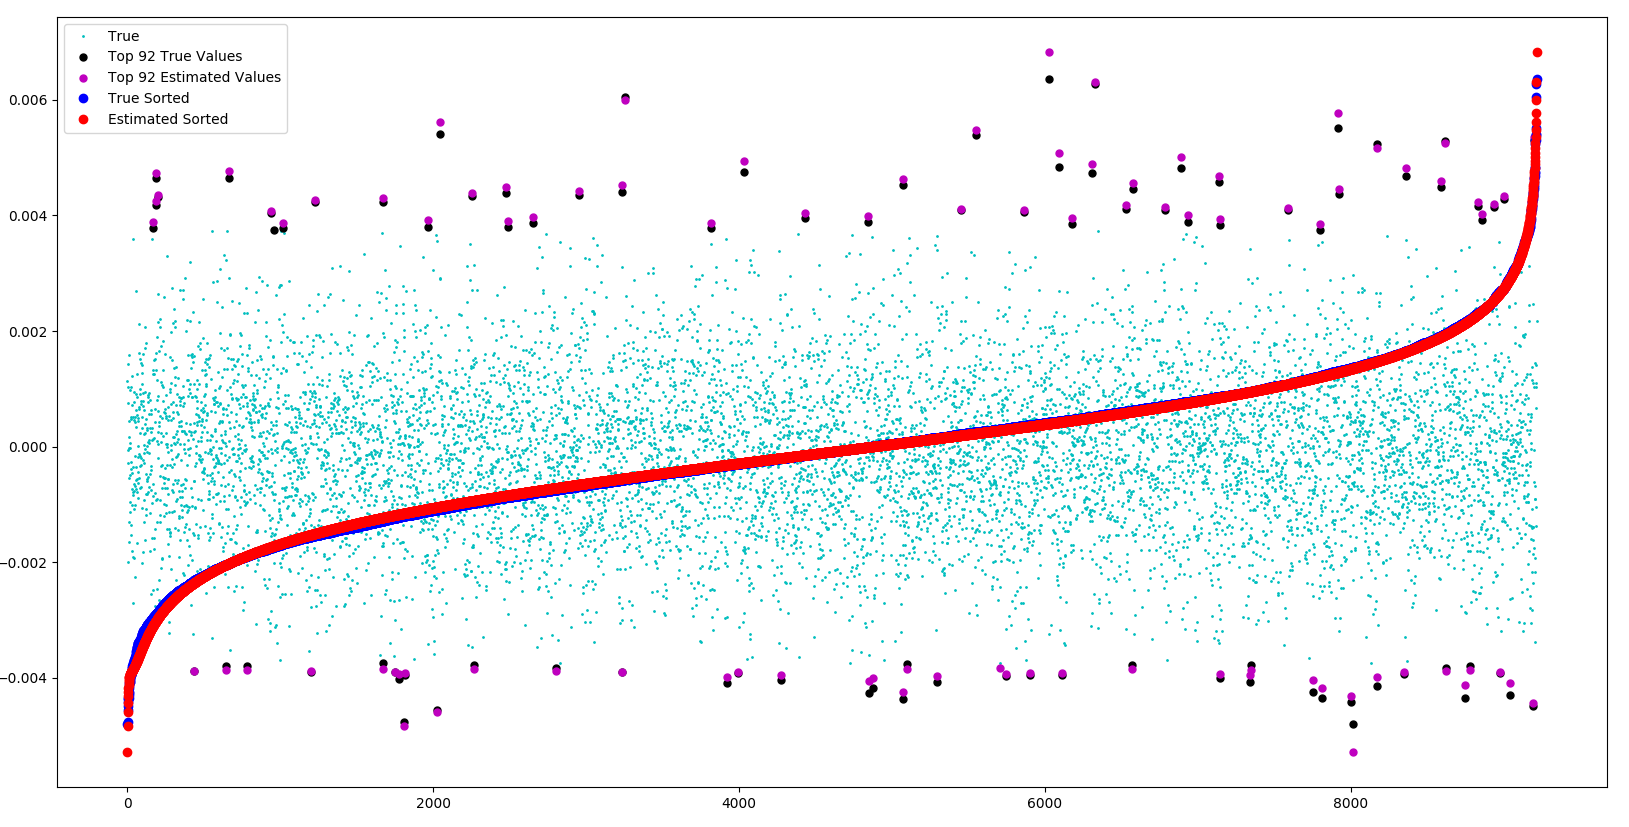
\includegraphics[width=1\textwidth]{figures/24gradient.png}
    \caption{Gradient Approximation using Logit basis functions}
    \label{logit}
    \end{figure}

    Parameterizing appropriately the basis functions was not an easy task. 
    It is a procedure that, ideally, should be automated and take place at runtime for every given gradient that is going to be compressed.
    This way the model will be more adaptive with respect to the form and characteristics of the gradients as those are produced during training.
    
    However, in this particular case, we selected the basis functions offline by experimenting on a collection of gradients that we sampled while training resnet20 on the cifar10 dataset.
    Consequently, the exact same set of basis functions would not produce good fits for the gradients of other models like vgg16 or densenet40.
    
    We provide more details regarding the training results in the "evaluation" section.
    
    \newpage
    \subsection{Fitting Curve Segments using polynomials}
    
    Another set of experiments was conducted by using functions of a polynomial form to fit different segments of the curve.
    In this case, we decided to first obtain the absolute values of $g$ and then apply sorting.
    The curve-segments would now look like those in figure \ref{segmented_29}.
    
    \begin{figure}[h]
    \centering
    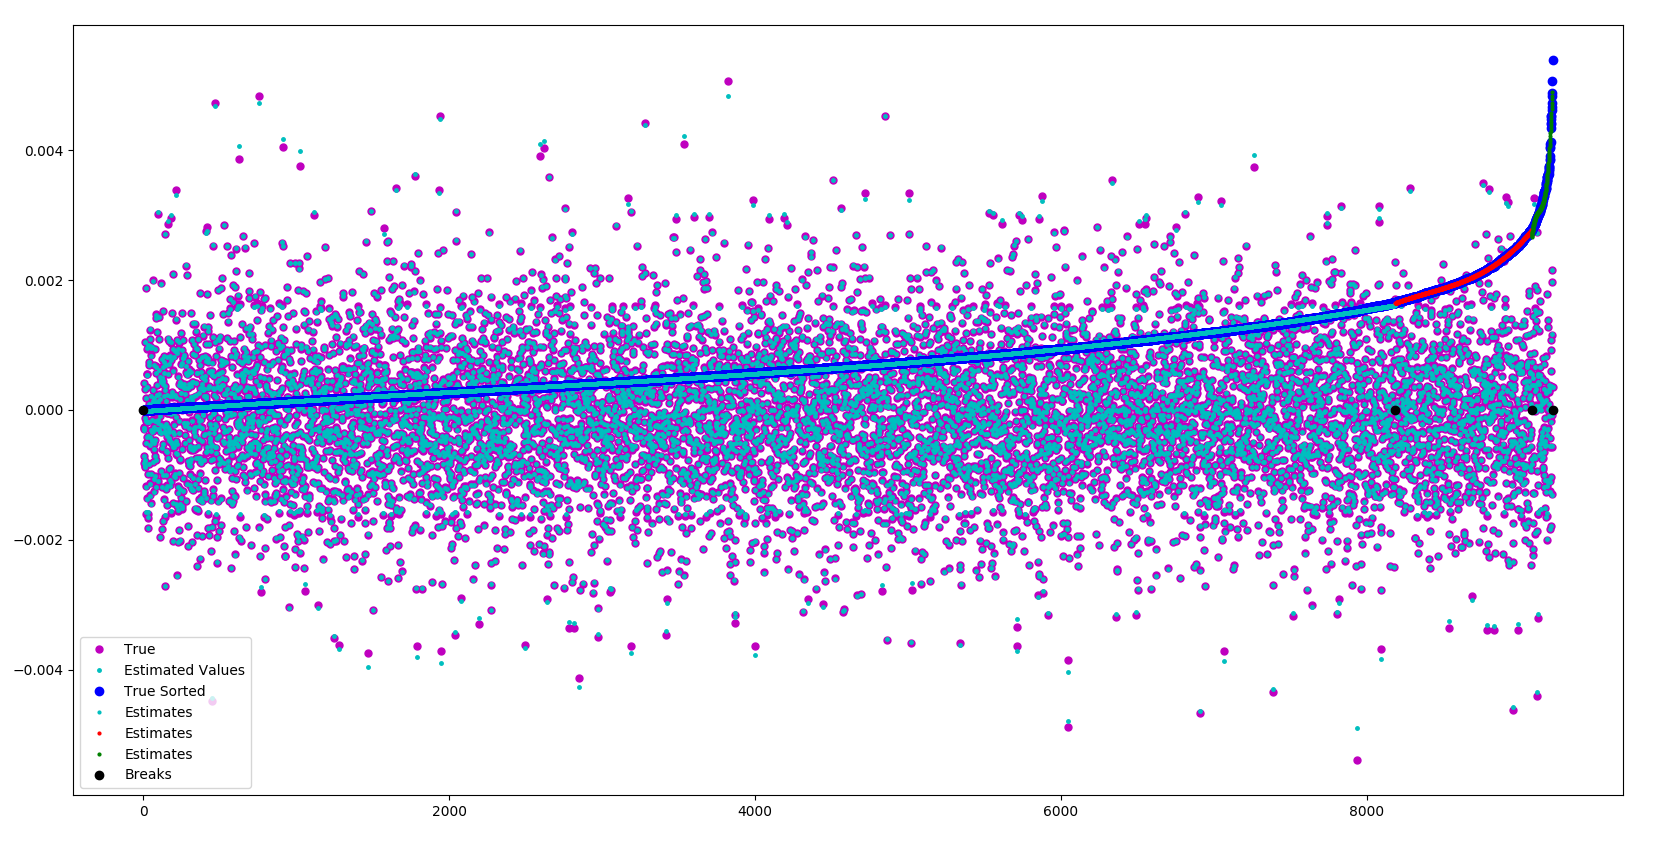
\includegraphics[width=1\textwidth]{thesis/figures/segmented_29gradient.png}
    \caption{Approximating Segments of the curve using Polynomial Basis Functions}
    \label{segmented_29}
    \end{figure}
    
    Again, both the number of curve-segments and the degree of each polynomial should be specified at runtime and adapt with respect to each gradient.
    However, in most cases we decide to explicitly define those values after some offline experimentation on the gradient samples. This relieves the workers from some additional computational overhead.
    Typically, extremely big gradients such as those produced by the VGG16 model (see figure \ref{vgg16-gradient}) would require a larger amount of segments for achieving good approximations.
    
    \begin{figure}[h]
    \centering
    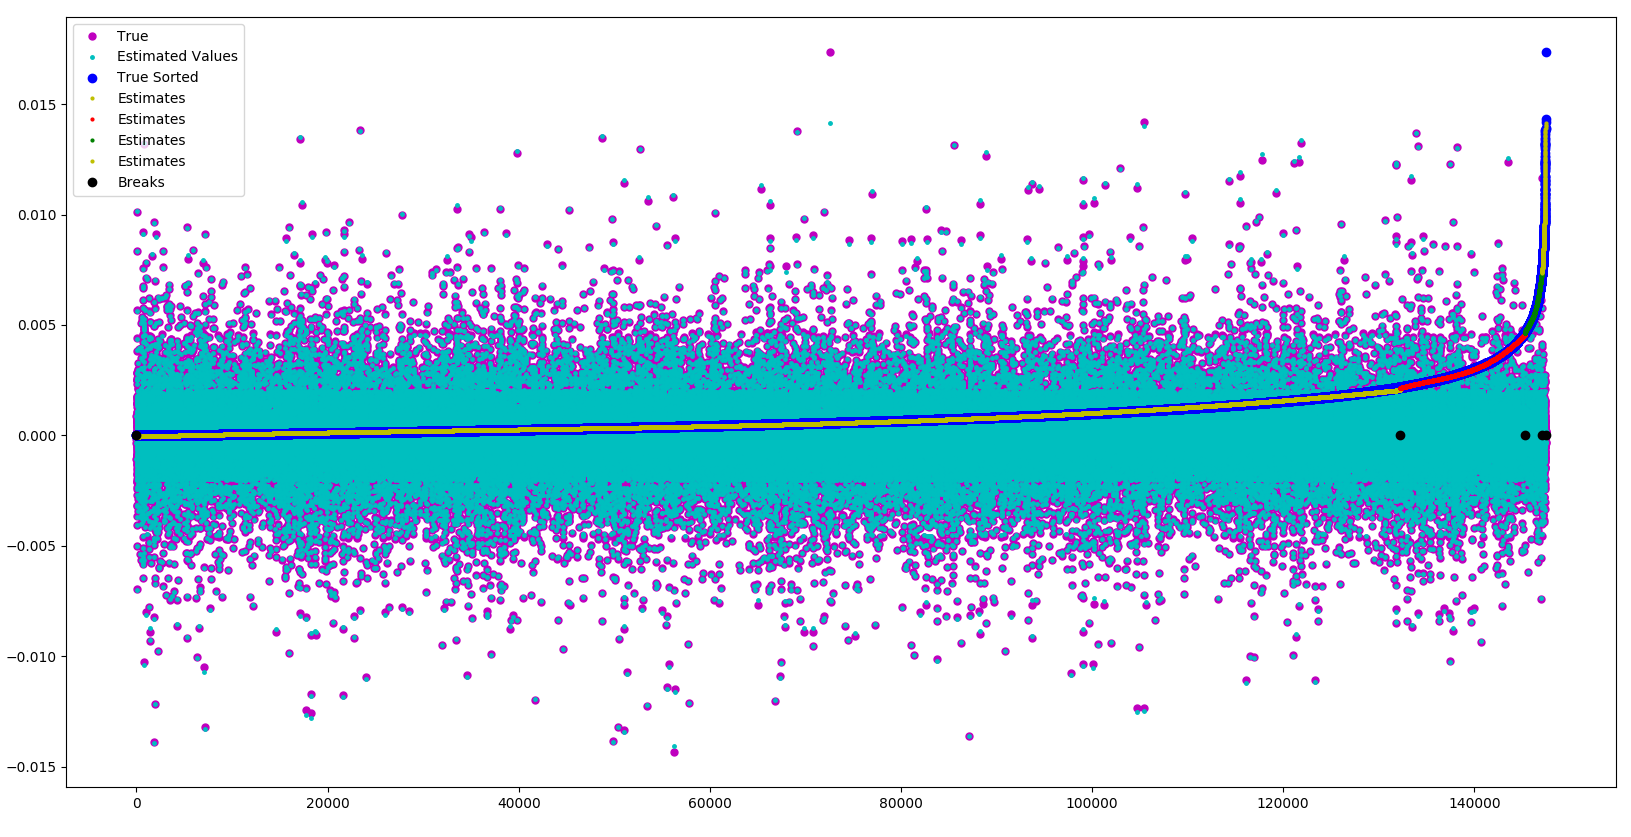
\includegraphics[width=1\textwidth]{thesis/figures/vgg16-6gradient.png}
    \caption{Fitting a VGG16 gradient using four curve-segments}
    \label{vgg16-gradient}
    \end{figure}
    
    Once again, we fitted the curve-segments using the LS method and employing a set of polynomials as basis functions (e.g. $X, X^2,\cdots,X^k$). 
    Contrary to other approaches, like the "double exponential" fitting that will be described next, cutting the curve into pieces and fitting them with polynomials helps us treat more peculiar cases of gradients, as the one in figure \ref{segmented_4}.
    You can see that, on the right part of this gradient, the curve-segment is an "anomaly" compared to the same segments of other similar gradients.
    
    \begin{figure}[h]
    \centering
    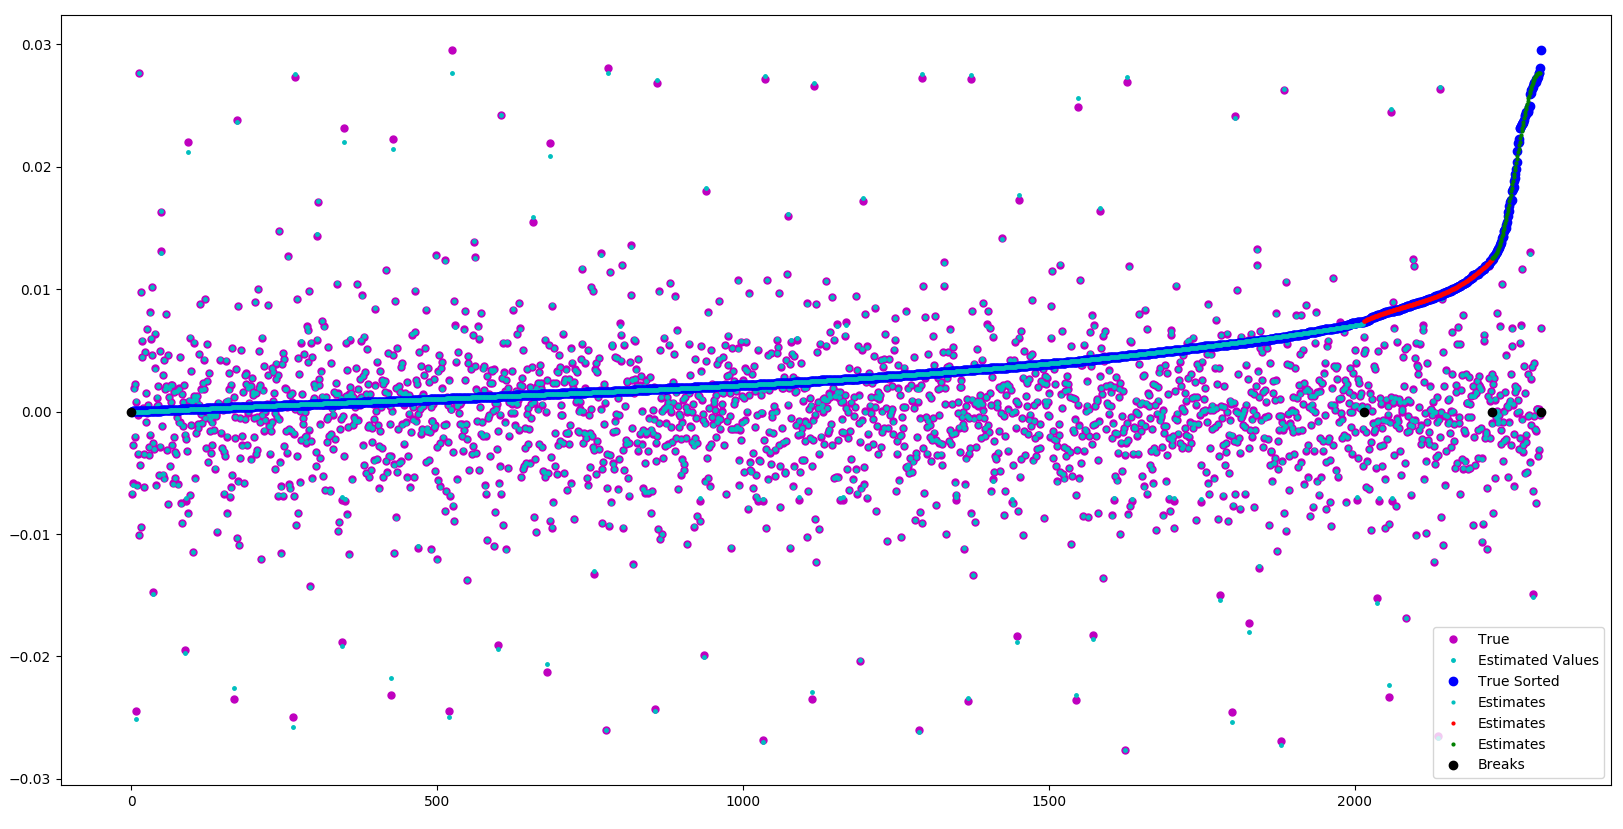
\includegraphics[width=1\textwidth]{thesis/figures/segmented_4gradient.png}
    \caption{}
    \label{segmented_4}
    \end{figure}

    Note that, the positive and negative values cannot be distinguished by the decompressor at this point. A way to resolve this it to integrate the sign information of each value in the mapping tensor. Now, every time a mapping index has a negative sign, the gradient value it corresponds to will have be negative as well.

    \section{Non-Linear Regression}
    
    As we previously mentioned, in linear regression the coefficients can only be linear.
    Non-linearity can be achieved by allowing the existence of non-linear coefficients in the functional form of the curve.
    
    For example, the following is a non-linear model:
    \begin{flushleft}
    \centering
    \setlength{\parindent}{40ex} 
    $\hat{y} = \hat{w_0} * \cos{(x+\hat{w_4})} +  \hat{w_2} * \cos{(2*x+\hat{w_1})} + \hat{w_3}$
    \end{flushleft}
    
    \subsection{Double Exponential Functions}
    
    Another parametric family we chose to include in our experiments was the following: 
    \begin{flushleft}
    \centering
    \setlength{\parindent}{40ex} 
    $\hat{y} = \hat{w_0} * e^{(\hat{w_1}*x)} + \hat{w_2} * e^{(\hat{w_3}*x)}$
    \end{flushleft}
    
    We call it "double exponential" and it is clearly non-linear in the coefficients. By employing the LS loss function we can obtain, once again, an analytical solution for finding the optimal coefficients.
    Similar to the polynomial approximations, we apply the curve fitting on the sorted, absolute values of the gradient $g$, as shown in figure \ref{double_exp}.
    
    \begin{figure}[h]
    \centering
    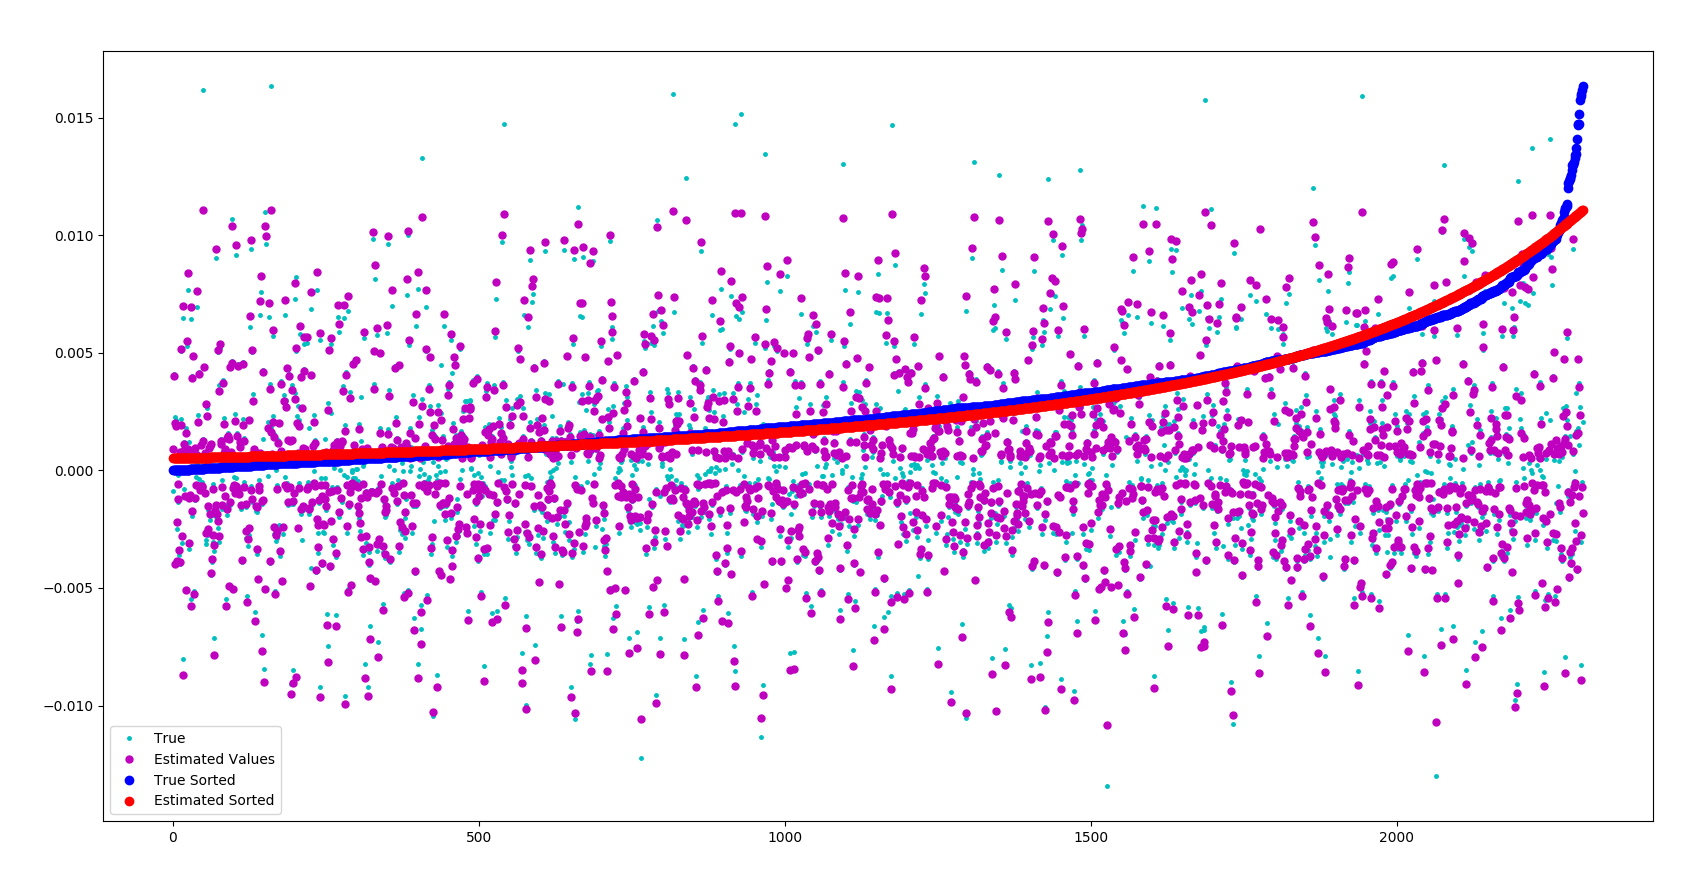
\includegraphics[width=1\textwidth]{figures/4gradient double_exp.png}
    \caption{Gradient Approximation using a double exponential}
    \label{double_exp}
    \end{figure}
    
    \section{Fitting the Sparsified Tensor Values}

    
    Now, any of the above methods can be applied on top of a sparsification method, like Top-r. The benefit of doing this is the reduction of the mapping tensor and thus the shrinking of the overall message.
    In figure \ref{topk-resnet-19gradient}, we used the "double exponential" method to fit the top-r values of the gradient, as shown on the right part of the plot.
    More details regarding the accuracy and throughput of the experiments will be provided in the evaluation section.
    
    \begin{figure}[h]
    \centering
    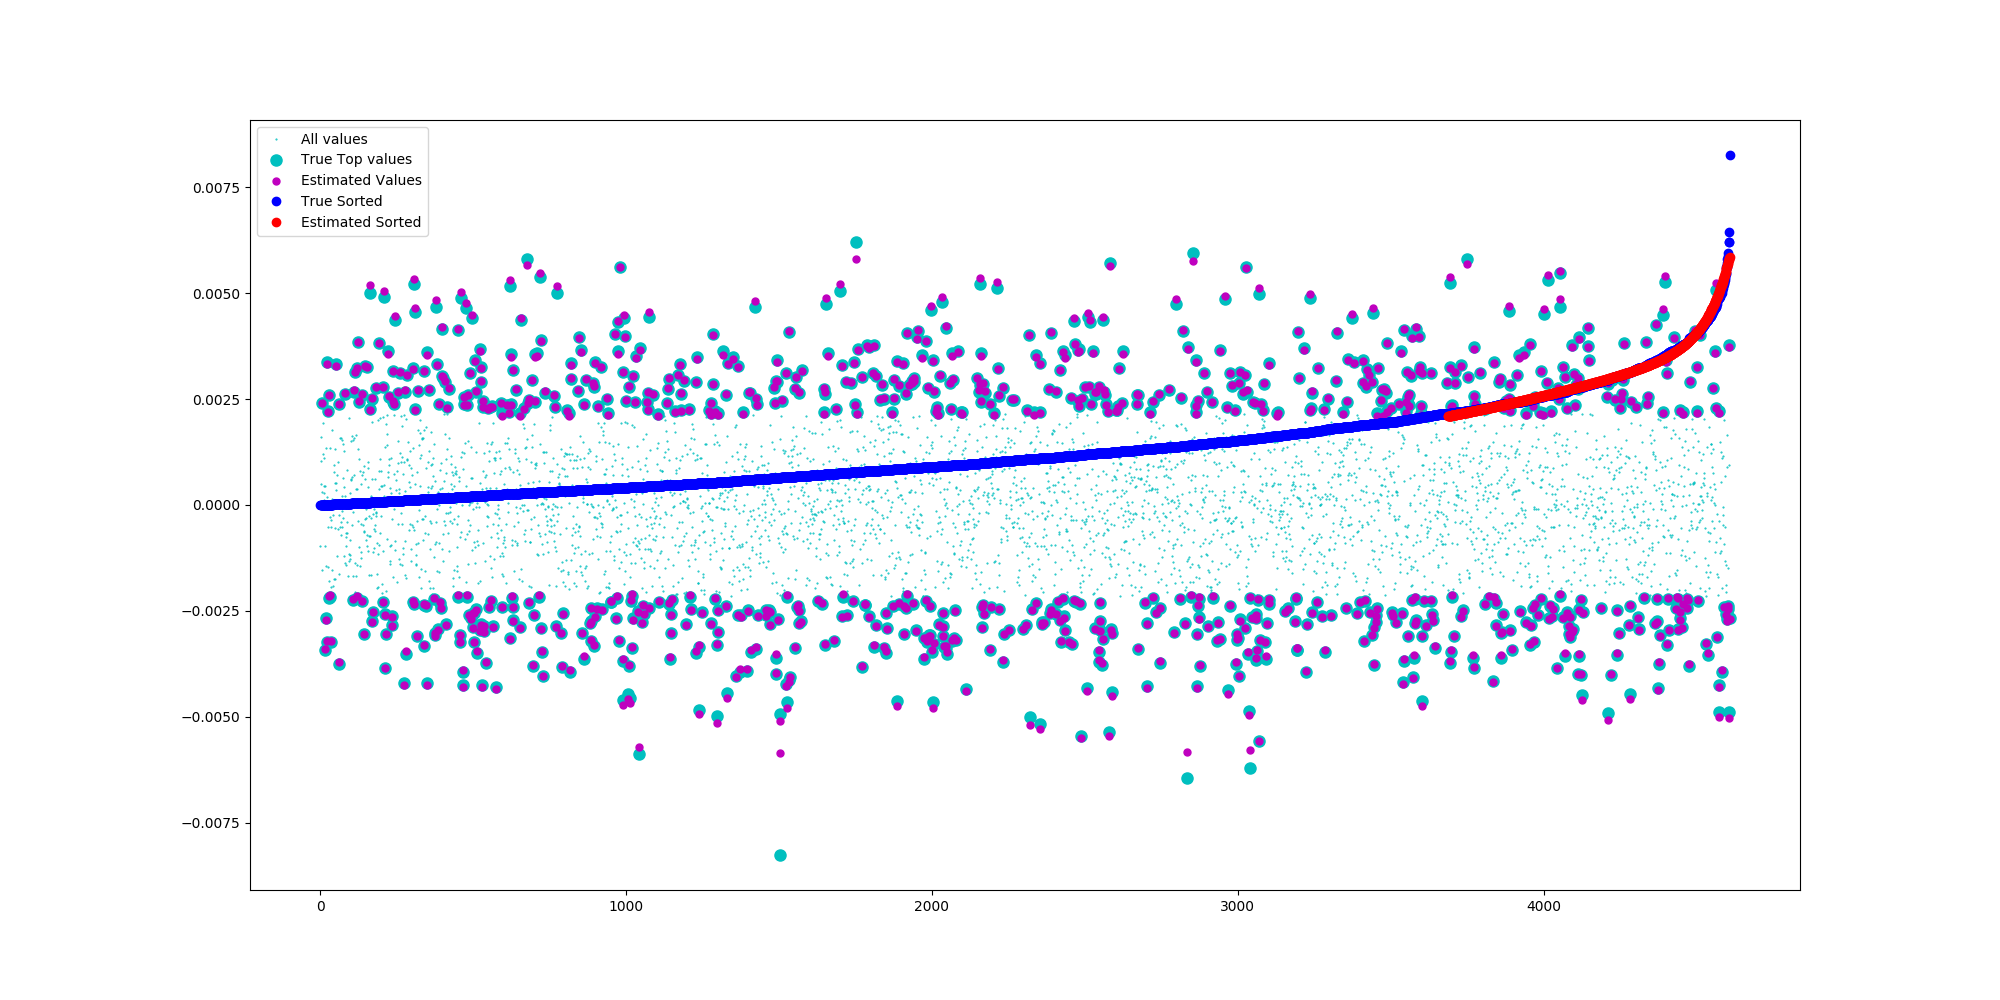
\includegraphics[width=1\textwidth]{thesis/figures/topk-resnet-19gradient.png}
    \caption{Gradient Approximation using a double exponential}
    \label{topk-resnet-19gradient}
    \end{figure}
    